%%
%% Copyright 2007, 2008, 2009 Elsevier Ltd
%%
%% This file is part of the 'Elsarticle Bundle'.
%% ---------------------------------------------
%%
%% It may be distributed under the conditions of the LaTeX Project Public
%% License, either version 1.2 of this license or (at your option) any
%% later version.  The latest version of this license is in
%%    http://www.latex-project.org/lppl.txt
%% and version 1.2 or later is part of all distributions of LaTeX
%% version 1999/12/01 or later.
%%
%% The list of all files belonging to the 'Elsarticle Bundle' is
%% given in the file `manifest.txt'.
%%
%% Template article for Elsevier's document class `elsarticle'
%% with harvard style bibliographic references
%% SP 2008/03/01

\documentclass[final,3p,times,twocolumn]{elsarticle}

%% Use the option review to obtain double line spacing
%% \documentclass[authoryear,preprint,review,12pt]{elsarticle}

%% Use the options 1p,twocolumn; 3p; 3p,twocolumn; 5p; or 5p,twocolumn
%% for a journal layout:
%% \documentclass[final,1p,times]{elsarticle}
%% \documentclass[final,1p,times,twocolumn]{elsarticle}
%% \documentclass[final,3p,times]{elsarticle}
%% \documentclass[final,3p,times,twocolumn]{elsarticle}
%% \documentclass[final,5p,times]{elsarticle}
%% \documentclass[final,5p,times,twocolumn]{elsarticle}

%% For including figures, graphicx.sty has been loaded in
%% elsarticle.cls. If you prefer to use the old commands
%% please give \usepackage{epsfig}

%% The amssymb package provides various useful mathematical symbols
\usepackage{amssymb}
\usepackage{amsmath}
\usepackage{epstopdf}
\usepackage{hyperref}
\usepackage{color}
\usepackage{multirow}

%% The amsthm package provides extended theorem environments
%% \usepackage{amsthm}

%% The lineno packages adds line numbers. Start line numbering with
%% \begin{linenumbers}, end it with \end{linenumbers}. Or switch it on
%% for the whole article with \linenumbers.
%% \usepackage{lineno}

\journal{Applied Acoustics}

\newcommand{\ml}[1]{\textcolor{blue}{ Mathieu: #1}}
\newcommand{\fg}[1]{\textcolor{red}{ Felix: #1}}

\begin{document}

\begin{frontmatter}

%% Title, authors and addresses

%% use the tnoteref command within \title for footnotes;
%% use the tnotetext command for theassociated footnote;
%% use the fnref command within \author or \address for footnotes;
%% use the fntext command for theassociated footnote;
%% use the corref command within \author for corresponding author footnotes;
%% use the cortext command for theassociated footnote;
%% use the ead command for the email address,
%% and the form \ead[url] for the home page:
%% \title{Title\tnoteref{label1}}
%% \tnotetext[label1]{}
%% \author{Name\corref{cor1}\fnref{label2}}
%% \ead{email address}
%% \ead[url]{home page}
%% \fntext[label2]{}
%% \cortext[cor1]{}
%% \address{Address\fnref{label3}}
%% \fntext[label3]{}


\title{A sensor grid approach for large scale acoustic monitoring}

%% use optional labels to link authors explicitly to addresses:
%% \author[label1,label2]{}
%% \address[label1]{}
%% \address[label2]{}

\author{F\'elix Gontier, Mathieu Lagrange, Pierre Aumond, Arnaud Can, Catherine Lavandier}

\address{felix.gontier@reseau.eseo.fr}

\begin{abstract}
%% Text of abstract

The acoustic environment represents both societal and environmental concerns. Monitoring the acoustic environnment in urban but also rural or wilderness areas is therefore an important matter. Fostering on the recent development of low cost hardware acoustic sensors, we propose to consider a sensor grid approach to tackle this issue.

In this kind of approach, the crucial question is the nature of the data that is transmitted from the sensors to the processing and archival servers. To this end, we propose an efficient audio coding scheme based on third octave band spectral representation that allows 1) the estimation of most acousitc indicators and 2) the recognition of acoustic events at state of the art performance rate. The former is useful to provide quantitative information about the acoustic environment, while the latter is useful to gather more qualitative information and build perceptually motivated indicators using for example some emergence of a given sound source.

The coding scheme is also demonstrated to transmit spectrally encoded data that, reverted to the time domain using state of the art techniques, is not intelligible, thus protecting the privacy of citizens.

\end{abstract}

\begin{keyword}

acoustic monitoring \sep soundscape assessment \sep
%% keywords here, in the form: keyword \sep keyword

%% PACS codes here, in the form: \PACS code \sep code

%% MSC codes here, in the form: \MSC code \sep code
%% or \MSC[2008] code \sep code (2000 is the default)

\end{keyword}

\end{frontmatter}

%% \linenumbers
\clearpage
%% main text
\section{Introduction}
%\label{}

The advent of low cost acoustic sensors together with the need to better monitor and comprehend the acoustic environment of urban and wilderness areas give rise to the deployment of experimental sensor networks such as the sonyc (wp.nyu.edu/sonyc) and cense (cense.ifsttar.fr) projects.

To do so, considering the so-called "sensor grid" approach  \cite{lim2005sensor,tham2005sensorgrid} has several advantages. The sensor grid approach put the focus on a) a distributed system of data acquisition with a large set of sensors, b) the production and storage of a large dataset, and c) its availability for intensive and open data analysis computation.

In our application setting, the requirements are the following. First,  the number of sensor nodes shall be extended as needed without having to change the hardware and software architecture, \textit{i.e.} the approach shall be scalable. Second, the nodes shall be energy efficient in order ot ease the deployment of the sensors grid to the desired topology, ideally autonomous. Third, the encoding scheme used to transmit the data from the sensor to the storage and processing servers shall be designed with care in order to ensure the privacy of the citizen. Lastly, the data stored shall be as rich as possible while remaining a low bitrate for efficient transmission and storage.

The data of interest is first acoustic indicators (LAeq, ...) and second the presence of sound sources of interest (bird calls, sirens, explosion, ...). The latter allow us to better assess soundscapes in terms of pleasantness and other perceptual indicators \cite{lavandier2006contribution, aumond2017modeling}. This detection step can respectively be operated online (on the sensors) or offline (on the data servers).

The former is efficient in terms of data storage as only the detection events are transmitted and is thus currently considered in several approaches \cite{defreville2006automatic, mydlarz2017implementation, mydlarz2015design}. Though, it requires the availability of computing resources on the sensors in order to perform the detection step which as of today's efficiency of hardware do not allow them to be autonomous using power sources like decent size solar panels. Furthermore, the detection is done once and cannot be recomputed during posterior analyses.

The latter scheme has several benefits. First, the sensor is much simpler and can thus be autonomous in terms of energy, easing the deployment of the network. Second, it allows researchers to gather large amount of data that can be post processed and studied further offline. Data can be re analysed following newer classification schemes or using new indicators.

However, transmitting the raw audio through the network has several disavantages, in terms of required bandwidth, storage capabilities and privacy. Thus, for transmission from the sensors to the storage unit, the data can be encoded in a more efficient way than lossy audio encoding standards \cite{pan1995tutorial} as the audio signal is not mandatory for the computation of the acoustic indicators and the features needed for event recognition. Also, as the data is transmitted using the network and stored, one must ensure that the intelligibility of potential speech utterances is lost during the coding process, in order to ensure the privacy of the citizens.

We thus propose in this paper a audio coding scheme specifically tailored for use in a sensor grid which has the following features. It is of low bitrate but still allows the computation of most of the standard acoustics indicators with high precision. As far as acoustic event detection is concerned, we report equivalent performance of several state of the art classification schemes from features computed using raw audio data and encoded data. Finally, according to preliminary perceptual evaluation, the proposed coding scheme very strongly degrades the intelligibility, thus ensuring citizen privacy.

In order to promote reproducible research, the coder as well as the experiments needed to generate the figures will be made available to the community. The remaining of the paper is organized as follows: Section \ref{sec:background} reviews the types of data that needs to be estimated using the transmitted data and Section \ref{sec:coder} describes the proposed encoding scheme. The experimental protocol designed to validate the proposed approach is described in Section \ref{sec:protocol} and results are discussed in Section \ref{sec:results}.


\begin{figure}[t]
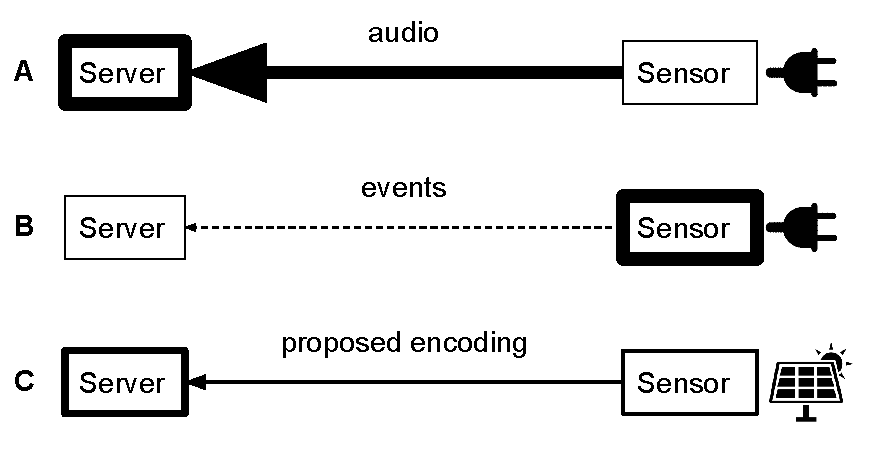
\includegraphics[width=\columnwidth]{figures/censeCoder}
\vspace{-0.15in}
\caption{Alternative implementations of the sensor grid approach for the monitoring of the acoustic environnment. In A) the raw audio is transmitted, in B) only the detected events, and in C) a compressed spectral representation. Thickness of arrows indicate bandwidth and thickness of boxes indicates the level of computation or storage required.}
\label{fig:codingScheme}
\end{figure}


\section{Background} \label{sec:background}


The present work is constrained to allow both acoustic monitoring and sound event recognition in urban soundscapes. Here we briefly review state-of-the-art methods in both subjects in order to better motivate our choices.

\subsection{Acoustic monitoring}

The considered sensor network primarily aims at monitoring urban soundscapes, that is, continously assessing their content and impact on the population. In the literature, this is typically enabled by measuring energetic acoustic indicators such as the equivalent sound pressure level $L_{eq}$ in dB SPL or its A-weighted equivalent $L_{Aeq}$ in dBA. However, while these indicators have proven to correlate well with perceptual evaluations for negative impact sound environments \cite{gozalo2015}, they are not sufficient to fully describe soundscapes \cite{rychtarikova2013}. Many other variables can be derived to better account for previously implicit properties \cite{can2016} including percentile values or time evolution. Studies have been conducted to select relevant subsets of descriptors in sound environment characterization \cite{can2015, brocolini2013, nilsson2007}.\\

All the mentionned indicators are measured at periods ranging from 0.125~ms or 1~s (resp. fast and slow) to longer periods of several minutes. Therefore, sound frequency information remains unused despite being closely related with subjective evaluations \cite{ishiyama2000}. A simple solution is the calculation of energetic indicators for the 31 third-octave bands within the human audition range 20~Hz - 20~kHz.\\

This measurement appears well-suited for this work's purpose: in addition to being an efficient descriptor \cite{torija2013}, it allows for the computation of most cited indicators while representing reasonably small, fixed amounts of data to be transmitted.

\subsection{Event detection}

Eventhough the above discussed indicators provide more richness than $L_{eq}$, recent studies show that abstract statistics are still not sufficient to fully model the human perception of soundscapes. The recognition of sources of interest is thus of importance. As far as the encoding scheme is concerned, it is thus important that the encoded data allows the computation of the above cited indicators but also the recognition of sources of interest with state of the art methods.

The recognition of sources of interest from audio streams has been the subject of extensive research in the past on speech \cite{anusuya2009}, music \cite{tzanetakis2002}, and lately more complex scenes in which the current work falls. Studied classification methods are diverse, ranging from time-dependant modeling with HMMs \cite{ntalampiras2014} to "bag-of-frames" approaches \cite{aucouturier2007, foggia2015}. Common architectures include learning-based classifiers such as support vector machines (SVM) \cite{kumar2016}, gaussian mixture models (GMM) \cite{radhakrishnan2005} or neural networks \cite{salamon2017, piczak2015}. However, the selection of relevant features is still an open debate. The most used are certainly spectral \cite{khunarsal2013} or cepstral \cite{couvreur2004} representations of the signal. Among them, mel spectrograms and their cepstral-domain derivation, the mel-frequency cepstrum coefficients (MFCC), are the most recurrent. These representations effectively try to model the human cochlear response to sounds by grouping frequency components around critical bands in a logarithmic scale, thus bearing important physical significance. They may also be exploited together with features computed in other domains to better model signal properties. For instance, \cite{cai2006} adds spectral features related to harmonicity and salient frequencies, and \cite{chu2009} uses a matching pursuit (MP) algorithm to deduce time-domaid features. Another promising solution is feature engineering via unsupervised learning, which \cite{salamon2015-2} implements with a k-means clustering technique. Alternative data representations such as the scattering transform \cite{bauge2013} show good results in environmental sound classification tasks \cite{salamon2015}.\\
A more detailed review of used methods is available in \cite{chachada2013}.

\section{Encoding scheme} \label{sec:coder}

The technical constraints of size inherent to the studied setup make it impossible to transmit raw audio recordings. Following the considerations briefly exposed in the previous section, we conclude that third-octave bands are a reasonable choice. As mentionned, they provide advantages in both acoustic monitoring quality and reduced data volume per measurement period. The physical content is also close to that of mel spectrograms, being just another filterbank transform with logarithmic frequency scaling.\\

A common way to implement third-octave analysis is to first design the highest octave three filters, and use them on progressively time-decimated versions of the input signal \cite{davis1986}. In practice, however, this technique presents multiple issues. \cite{antoni2010} presents an alternative analysis method based on direct frequency weighting. The weights matrix design procedure complies with both ANSI S1.1-1986 \cite{citeulike:9580295} and IEC 61260-1:2014 \cite{iec-norm} standards. It also respects the partition of unity principle over all frequency bins in the relevant range. Resulting filters for different parameter $l$ values are compared with Couvreur's implementation \cite{couvreur} of the time-domain filtering, as shown in Figure~\ref{fig:freq_filt}. The major difference is that gains at cutoff frequencies are fixed at the optimal -3dB by design.\\

\begin{figure}[htbp]
	\centering
		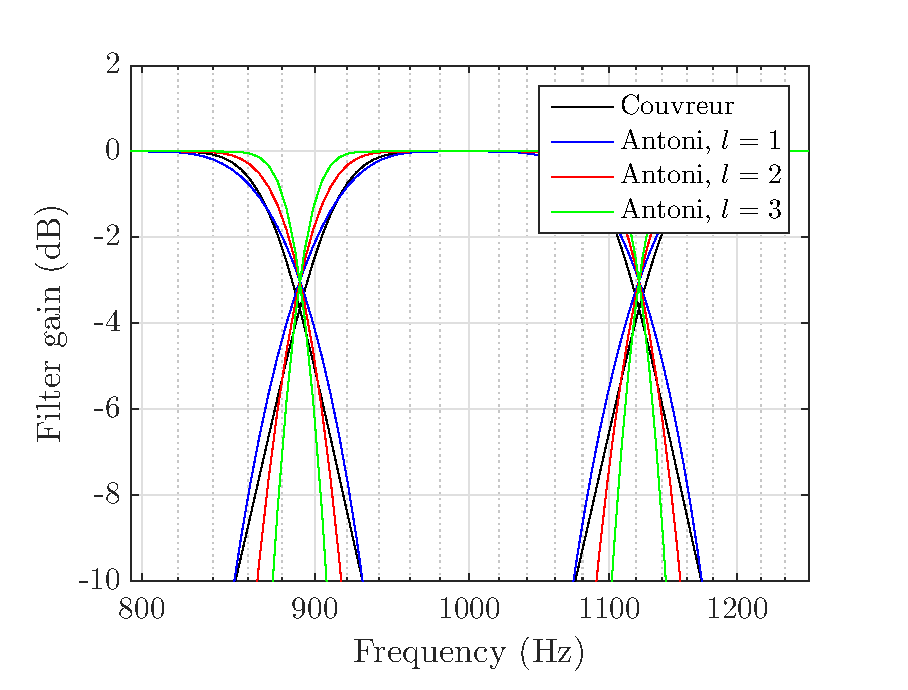
\includegraphics[width=\columnwidth]{figures/tob_imp.eps}
	\caption{Comparison of Couvreur's and Antoni's implementations of third-octave filters. Frequency-weighting allows for arbitrary transfer functions and thus more accurate gains as standards impose.}
	\label{fig:freq_filt}
\end{figure}

The first step is to represent the signal in the frequency domain using a short-term Fourier transform (STFT). The continuously sampled audio is segmented into 125~ms frames to provide "fast" acoustic measurements. The data is zero-padded to the next power of two to allow best fft performances. No overlap is used as it doubles both computational and memory costs and is not required for our application. A rectangular window is thus applied to ensure energy conservation in a given analysis frame. The phase is unimportant to third-octave analysis, thus it is discarded. Similarly, negative frequency components contain the same information as positive ones because the base signal is real. We then compute third-octave bands from the squared spectral magnitude by matrix multiplication with the frequency weights proposed in \cite{antoni2010} for $l = 2$\footnote{When implementing said method, we found that squaring the $\phi_l(p), l \geq 1$ intermediate function (p. 887) was the correct approach to meet cutoff frequencies requirements, and we believe this was the author's original intention.}. We include analysis for bands $i$ from -17 to 13, ie. center frequencies $f_i$ ranging from $20~Hz$ to $20~kHz$ with $f_0 = 1~kHz$. This means the main representation is composed of 31 values sampled every 125~ms.\\

Alternatively, we also implement the mel filterbank for comparison purposes, as the mel filterbank is the root representation of many state of the art classification algorithms. Mel spectrograms can thus be used as a baseline method to evaluate the relative performance of third-octave bands in sound event recognition.

As the Mel representation is not bounded by constraints such as conservation of energy, specific framing parameters or fixed resolution, it also offers a more flexible tool to study intelligibility alteration and coder performance, both of which we take interest in.

Mel spectrograms are computed with the \textit{rastamat} library \cite{ellis2005}. STFT analysis frames are obtained by applying a Hann window on 23.2~ms of signal with 50\% (11.6~ms) overlap to allow for efficient phase recovery in further tests.

\subsection{Data Encoding}

A Huffman coding scheme \cite{huffman1952} is then used to further reduce data dimensionality. As in most entropy coding algorithms, the efficiency of this technique depends on two important factors. A reduced amount of symbols in the dictionnary yields smaller code size on lower probability symbols. Lower data entropy, ie. lower average information content of the signal distribution, also increases performance. The first is generally obtained by applying a quantization process to the signal, whereas the second is directly linked with the probability density function (PDF) of these symbols. It is defined as $H = -\sum\limits_i p_ilog_n(p_i)$, where $p_i$ is the probability of appearance of a given symbol and $n$ the numerical base in which information is represented.

As such, entropy decreases when very few symbols have a very high probability of appearance and is maximum for a uniform distribution. Considering an estimated PDF for our data as shown in Figure~\ref{fig:pdf}a, immediately applying a linear quantization clearly results in most of the information being lost. We therefore spread the PDF by taking the logarithm of the representation. A linear quantization is then applied with $2^{q-1}-1$ output values to obtain Figure~\ref{fig:pdf}b. Finally, we use a $\Delta$-encoding algorithm along the time dimension to reduce redundancies. This also effectively concentrates higher probabilities on symbols around zero (Figure~\ref{fig:pdf}c). This yields a higher amount of symbols at $2^q-1$ but a nevertheless smaller entropy.

In the example shown here, the former is $H_{log} = 6.24~sh$ and the latter $H_{\Delta} = 3.54~sh$. Huffman encoding is then computed with either a frame-specific symbol-code dictionnary or a constant one generated from an entire dataset. A comparison of both methods is shown in Figure~\ref{fig:dict_comp}. For most short texture frame durations, we found the local Huffman algorithm to be much faster. In fact, encoding complexity is function of the amount of dictionnary elements. If it is specific to a given data packet, then it does not need to contain every possible value. This gain seem to outweight the additional complexity induced by the tree generation algorithm. Alternatively, short texture frames or single analysis windows can be encoded using one general dictionnary to improve bitrate. This choice depends on which of the size and complexity parameters must be reduced most.\\

\begin{figure}[htbp]
	\centering
		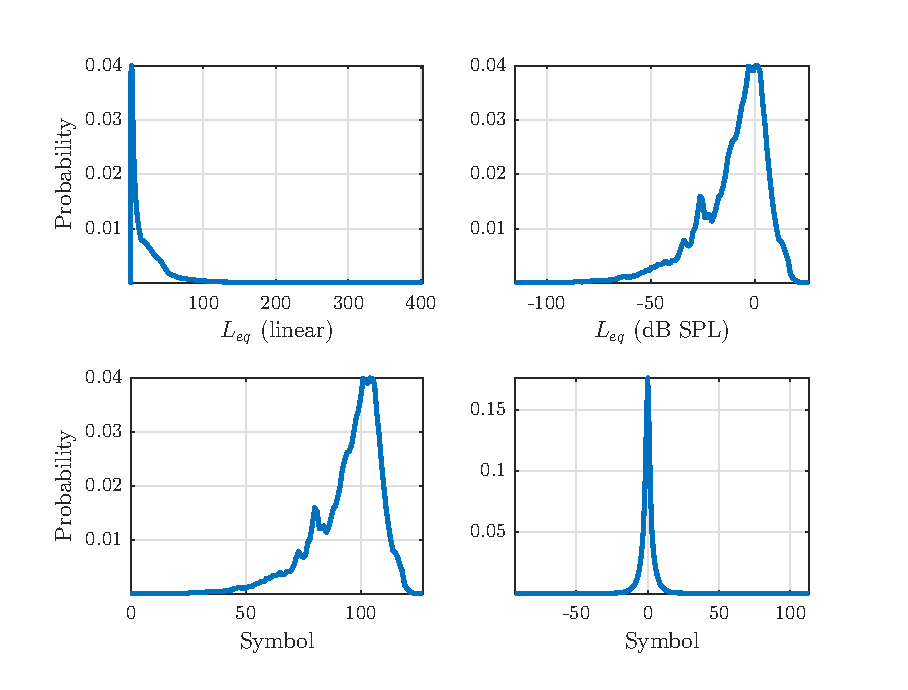
\includegraphics[width=0.5\textwidth]{figures/pdf.eps}
	\caption{Example of estimated probability density functions of the data throughout the encoding step. (left) Unchanged output of the representation step, concentrated towards very low values. (middle) PDF "flattening" effect induced by logarithm application. Here values are mapped to the range $[0, 2^7-1]$ and rounded to perform quantization. (right) Output of the $\Delta$ compression, with desirable probabilities as the input to a Huffman algorithm.}
	\label{fig:pdf}
\end{figure}

\begin{figure}[htbp]
	\centering
		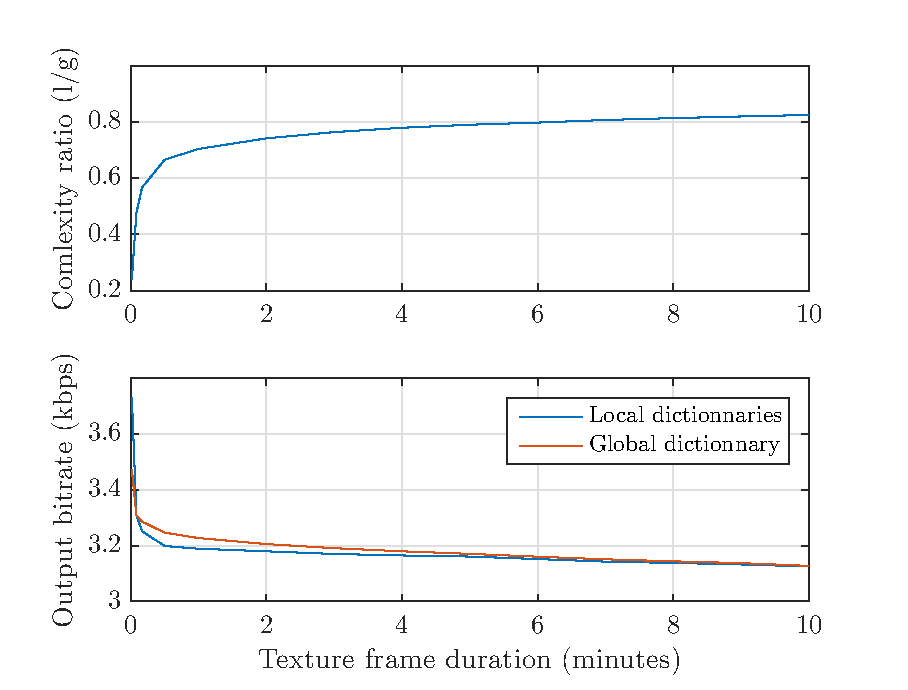
\includegraphics[width=\columnwidth]{figures/dict_comp.eps}
	\caption{Performance comparison of locally and globally generated Huffman dictionnaries. (top) The mean execution time ratio favors the use of frame-specific dictionnaries for tested texture frame lengths. (bottom) The mean output bitrate is close for both algorithms, showing that the necessity of sending symbol-code pairs mostly compensates for their optimality.}
	\label{fig:dict_comp}
\end{figure}

The decoding process is quite straightforward, as both Huffman and $\Delta$ compression are lossless and directly reversible. The entire coder scheme is summarized in Figure~\ref{fig:scheme}.

\begin{figure*}[htbp]
	\centering
		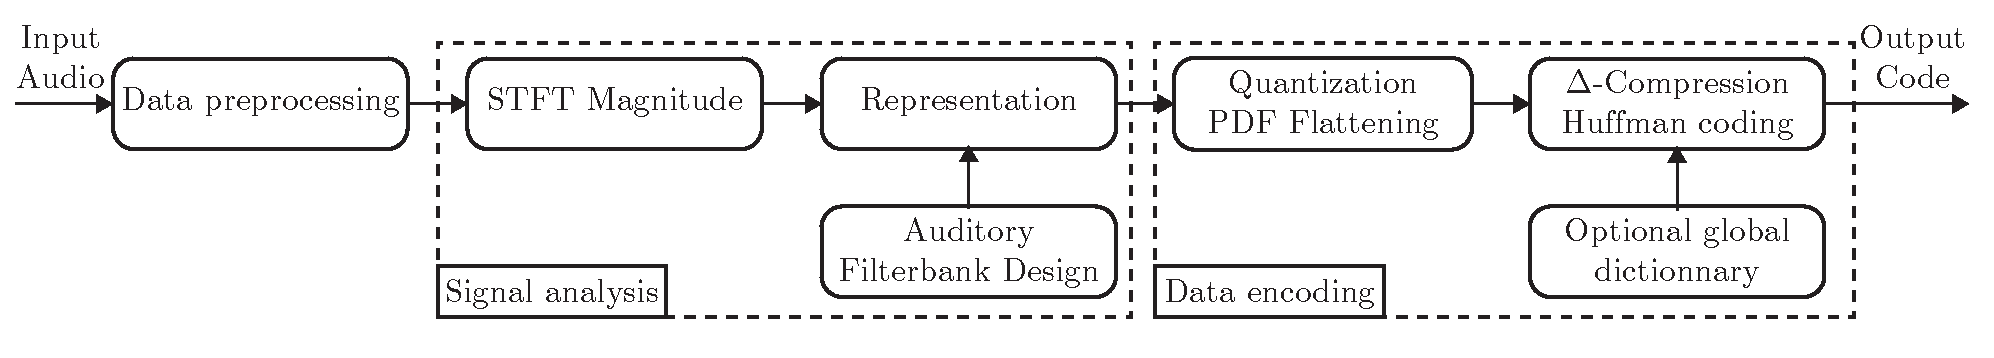
\includegraphics[width=1\textwidth]{figures/scheme.pdf}
	\caption{Overview of the coder process.}
	\label{fig:scheme}
\end{figure*}

\section{Validation protocol} \label{sec:protocol}

A set of metrics is computed to assess the efficiency of the proposed coder scheme and determine the impact of the algorithm's parameters, which are as follow: the desired word size prior to Huffman encoding, set by quantization for both signal representation choices, and only for Mel bands the number of coefficients between 10 and 40. We also study the effect of time averaging analysis frames: to force a fixed amount of frames per second lesser than the average speech rate in phonemes per second is a possible way to alter intelligibility at the cost of temporal information resolution.

\subsection{Efficiency}

The coder's output bitrate as well as additional measurement error is computed for both data representations : third-octave and Mel. It is expressed in dB and compared to the IEC 61672-1:2013 standard \cite{iec-norm2} on sound level meter tolerance. This is to verify that the quantization step yields a maximum absolute error inferior to the precision of the target recording device. To provide relevant statistics, these quantities are estimated for a total of 53 10-minutes texture frames. They are obtained from the UrbanSound8k dataset presented in the next section.

\subsection{Event recognition}

In order to ensure that the proposed scheme allows the recognition of events using state of the art methods, we consider the UrbanSound8k dataset\cite{salamon2014}. It features about 9 hours of urban environmental sounds recordings separated in 8732 wave files ranging from 1 to 4 seconds each. The recordings are labeled in 10 classes (air conditioner, car horn, children playing, dog bark, drilling, enginge idling, gun shot, jackhammer, siren, street music), and distributed in 10 independant folds. A method and baseline results are also provided for the classification task. It is used in all the following experiments with the exception of intelligibility computation for which a small dataset of high-quality voice recordings is preferred. Audio files are resampled 44.1~kHz, normalized and reduced to a single channel.\\

We evaluate the global loss of information by implementing the four classification models proposed in \cite{salamon2014}: a support vector machine with a radial basis function kernel, a random forest classifier with 500 trees, a decision tree and a k-nearest neighbors classifier with $k = 5$. Values for the SVM parameter $C$ and RBF kernel variance $\sigma^2$ are found with a grid search. We apply a discrete cosine transform to the critical band signal representation to obtain cepstra (known as Mel Frequency Cepstrum Coefficients or MFCC in the first case) of which we conserve the 25 first coefficients, and summarize along time with the mean, variance, skewness, kurtosis, minimum, maximum, median, derivative mean and variance, second order derivative mean and variance. The feature vector is thus comprised of 275 values to reproduce available results and compare with our own. Models are trained for each setup using a 10-fold cross validation method provided by the authors of \cite{salamon2014}, that is, every combination of testing one fold on models trained with the other nine.

\subsection{Inintelligibility}

Intelligibility in decoded and reconstructed audio is also oan concerns of this study. It is indeed important that the produced scheme maintains a high level of recognition of acoustic events but, as the dat is transmitted over the network and potentially stored, the level of intelligibility of the decoded stream should be as low as possible.

%conduct thus preliminary perceptive tests to ensure that a clean speech recording is made unintelligible, implying the same results in usually noisier urban soundscapes. We also

We thus provide the computation of two objective metrics: the Coherence Speech Intelligibility Index\cite{kates2005} (CSII) and frequency-weighted segmental SNR\cite{hu2008} (fwSNRseg) by comparing original unaltered samples and recovered audio. These two indicators have been shown to correlate well with perceptual tests\cite{ma2009}, although results are only available for lesser degradations and distortions than the ones we consider in this study.\\

These metrics require a recovery of the time-domain signal. To do so, a linearly-scaled spectrogram from the band-focused representations is estimated. This estimation can be achieved by multiplying by the scaled transpose of the forward transformation matrix. A loss of resolution increasing with frequency is induced due to the shape of the transformation, as illustrated by Figure~\ref{fig:freq}. Signal phase is approximated by either white noise spectrogram scaling or a Griffin \& Lim algorithm \cite{griffin1984}, and the signal is retrieved using concatenation or overlap-add. When using overlap to compute third-octave bands, one can also avoid framing effects produced by rectangular windowing by convoluting the signal with another windowing function prior to inverse-STFT computation.\\

\begin{figure}[htbp]
	\centering
		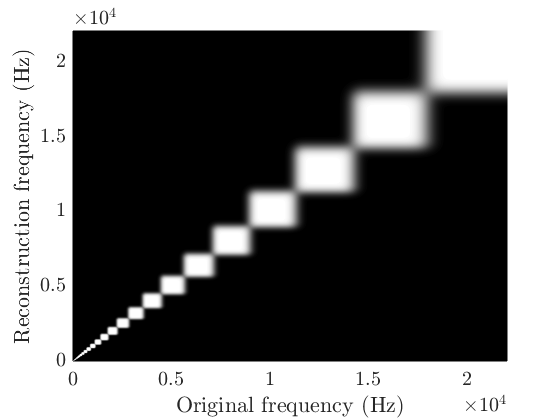
\includegraphics[width=\columnwidth]{figures/freq.png}
	\caption{Third-octave bands analysis and approximate inverse transformation effects on energy location. This process yields an important and heterogeneous loss in resolution, particularly at higher frequency points.}
	\label{fig:freq}
\end{figure}



\section{Results} \label{sec:results}

\subsection{Coder efficiency}

The main indicator of performance is the bitrate obtained at the output of the coder. The three varying factors studied are the data word size $q$, the number of bands and the effect of reducing time-resolution by averaging analysis frames. Figure~\ref{fig:bitrate_q} shows estimations of the output bitrate for different values of $q$. To match third-octave bands computation principle where a 125~ms analysis is mandatory, we averaged mel frames over time. Because we use the most common parameters, namely 23.2~ms window with 50\% overlap, the closest achievable rate considering simple averaging is 7.74 frames per second. Third-octave representation on 31 bands yielded an overall higher size than their mel equivalent, here estimated for 30 bands. It however compares with the 40-mel bands representation which is the most used in litterature. This occurence is likely due to the distribution observed by the data prior to Huffman encoding.

\begin{figure}[htbp]
	\centering
		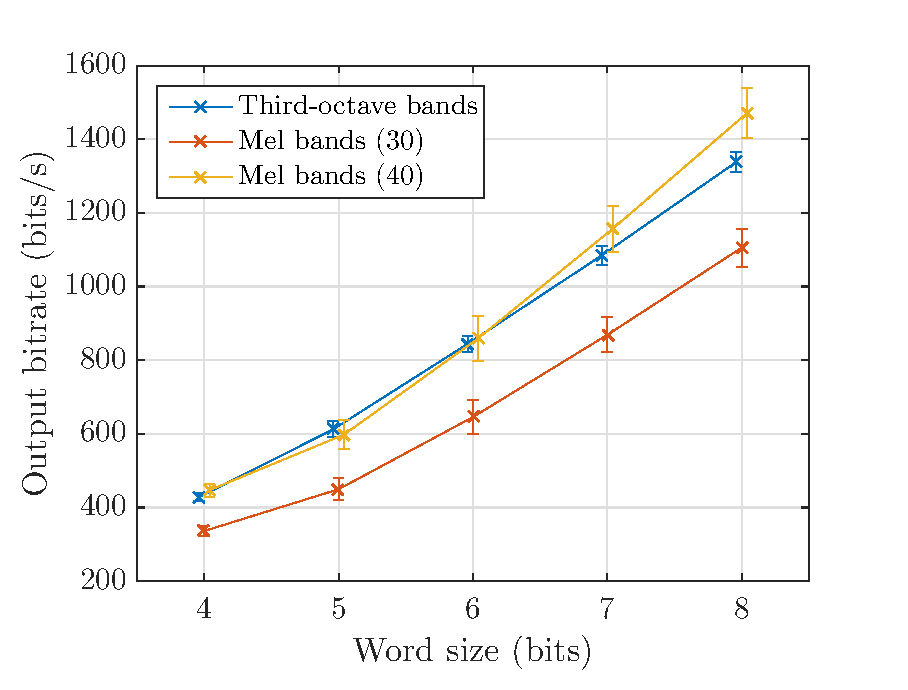
\includegraphics[width=\columnwidth]{figures/bitrate_qall.eps}
	\caption{Coder output bitrate as a function of quantization for third-octave and mel bands with 8 frames per second.}
	\label{fig:bitrate_q}
\end{figure}

A second set of parameters influences directly the time-frequency resolution of the analysis. By choosing a frame rate and number of bands, one can effectively control the size of periodically transmitted data. We evaluate the bitrate for 10 to 40 mel bands and a frame rate from 2 to 10 per second, with fixed $q = 8$. Results are exposed in Figure~\ref{fig:bitrate_mel_avg}. As expected, the bitrate for a given word size $q$ can be modeled as a linear function of the representation dimensions for one second of analysis. Small variations are induced by data distributions on a per-frame level and their effect on the Huffman algorithm.

\begin{figure}[htbp]
	\centering
		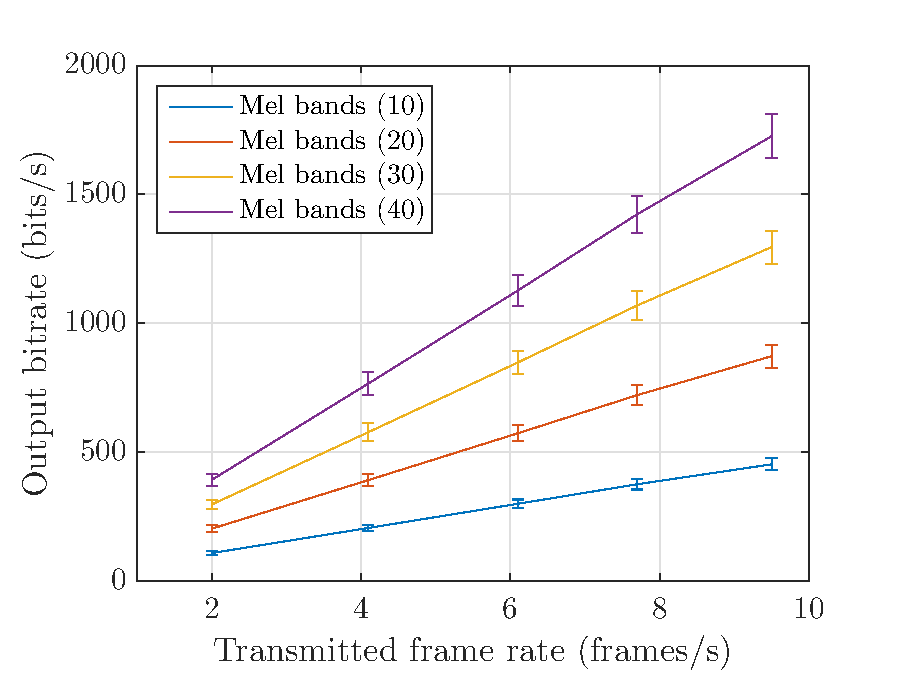
\includegraphics[width=\columnwidth]{figures/bitrate_mel_avg.eps}
	\caption{Impact of representation resolution on the encoded data bitrate.}
	\label{fig:bitrate_mel_avg}
\end{figure}

This experiment aims at assessing potential tradeoffs between bitrate and information. As such, it will be further discussed in the \textit{Event recognition} subsection.\\

We also examine the additionnal error caused by the encoding steps after obtaining the desired data representation. The only lossy operation applied is quantization, which is defined by an output word size $q$ in bits. However, it corresponds to the word size \textit{after} $\Delta$-compression, meaning that the data is in fact quantized on $2^{q-1}$ values. Since these measurements are already expressed in dB, the error $\varepsilon$ is:
\begin{equation*}
	\varepsilon = |x_q-x|
\end{equation*}
where $x_q$ and $x$ are the quantized and clean representations repectively. $x_q$ is given by:
\begin{equation*}
x_q(n) = \frac{\Delta_x}{2^{q-1}-1}\textrm{round}\left(\frac{(2^{q-1}-1)x(n)}{\Delta_x}\right), x\in \left[0, \Delta_x\right]
\end{equation*}
Figure~\ref{fig:error_q} shows an estimation of $\varepsilon$ as a function of $q$ for third-octave and mel bands. In both cases, the mean and standard deviation seem to decrease by a factor of 2 as $q$ increases. To explain this phenomenon, let us model $x$ as a uniform distribution such as $x\sim \textit{U}\{0, \Delta_x\}$. While this is not exact it matches our objective when using a logarithm to flatten given PDFs. The error $\varepsilon$ will follow a uniform distribution $U\sim \{0, \frac{\Delta_x}{2\times (2^{q-1}-1)}\}$. Therefore, the mean and standard deviation are:
\[
\begin{cases}
	\mu_\epsilon = \frac{\Delta_x}{4\times (2^{q-1}-1)}\\
	\sigma_\epsilon = \frac{1}{12}\frac{\Delta_x}{2\times (2^{q-1}-1)}
\end{cases}
\]
justifying the decaying ratio as $q$ increases. In practice, we assume that $\varepsilon = f(\Delta_x, \frac{1}{2^{q-1}-1})$ with the heterogeneity of the data's PDF inducing small variations.\\

\begin{figure}[htbp]
	\centering
		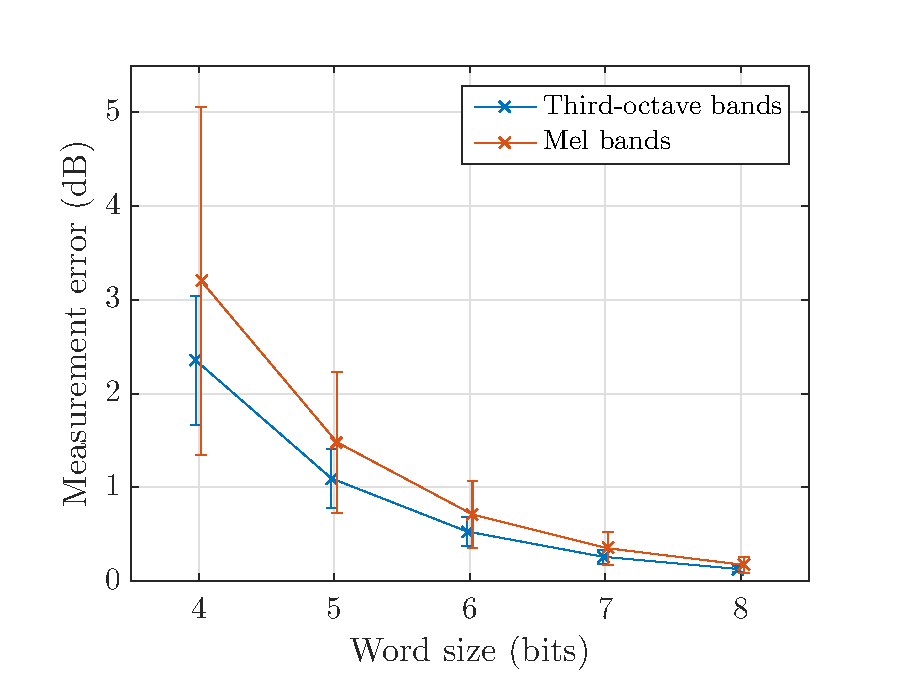
\includegraphics[width=\columnwidth]{figures/error_qall.eps}
	\caption{Measurement error induced by encoding for different quantization resolutions.}
	\label{fig:error_q}
\end{figure}


As $\Delta_x$ is sampled for each analysis frame in our implementation, the error has the same statistics across all bands. We compare the observed values against those specified in the IEC 61672-1:2013 \cite{iec-norm2} for $f = 1~kHz$ as it is where the most accurate measurements are expected. For class 1 and 2 sound level meters, the tolerance is set at about $\pm 1~dB$ and $\pm 1.5~dB$ respectively. Results for 6, 7 or 8-bit words lie within the shorter range and are therefore compliant with those standard's measurement tolerance.

\subsection{Event recognition}

The same set of parameters as in bitrate evaluation is used to study the impact of their tuning to the sound event recognition performance. We thus aim at finding ways to further reduce the encoded data size without strongly affecting recognition performance. Results of the four presented classification methods are provided for the sake of completeness.\\

First, we observe the impact of quantization on classification accuracy. The models are trained on the most complete implemented representation, ie. 40 mel bands and no time averaging (85 frames per second). Figure~\ref{fig:class_mel_q} shows that this process yields equivalent accuracy for higher resolutions.\\

\begin{figure}[htbp]
	\centering
		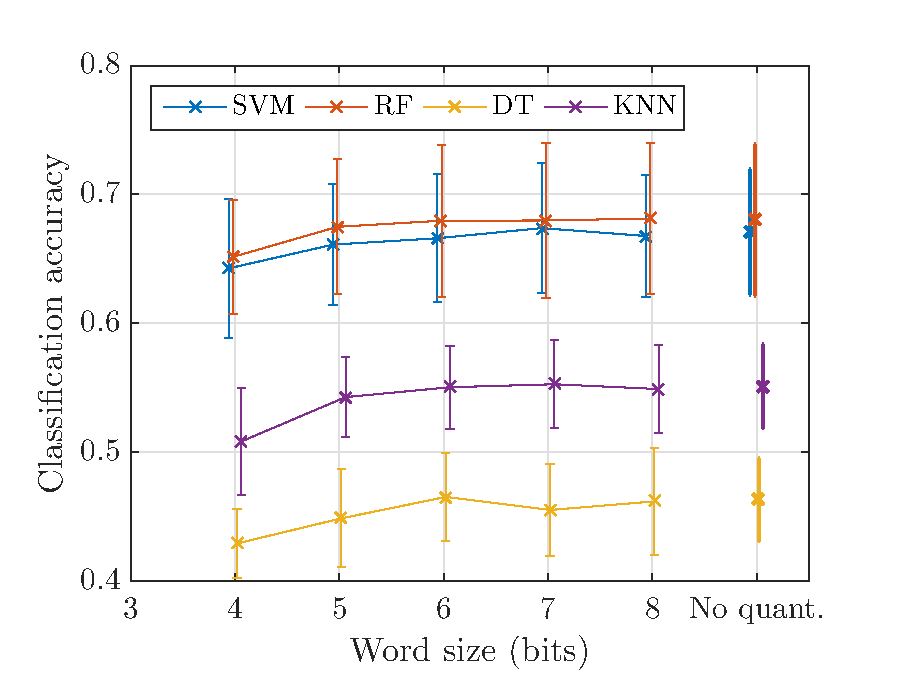
\includegraphics[width=\columnwidth]{figures/class_mel_q.eps}
	\caption{Classification accuracy as a function of word size before encoding. The baseline on the right is computed without quantizing the representation.}
	\label{fig:class_mel_q}
\end{figure}

The effect of changing representation time-frequency resolution is presented in Table~\ref{T1}. Similarly to baseline results, the random forest and SVM classifiers are the higher performing systems at $0.69\pm 0.06$ and $0.68\pm 0.04$ respectively. However, we find that given our setup, diminishing the number of analysis bands to some extent most often does not induce a strong drop of performance. The performance of the decision tree classifier is a good example of this behavior, with best performances for 10 mel bands only and a 4\% lower accuracy for 40. Even if the difference is small, all other models perform best with 30 or 40 mel bands as a representation. Time decimation is also possible, as the original representation can be averaged and consistently yield a good classification accuracy. The loss of information can be considered negligible for FPS values as low as 20 or 10 depending on the method. Even below, classification accuracy only drops by one or a few percents. This means that we can effectively divide the data size by a factor of at most 10 without affecting sound event recognition performance. It also provides us with a preliminary confirmation of the possibility for "fast"-sampled third-octave bands cepstra to match  MFCC performances.\\

\begin{table*}[h]
\centering
\caption{Classification accuracy in percentage for different classifiers: SVMs (a), Random Forests (b), Decision Trees (c), and Nearest Neigbors (d) with respect to varying representation resolutions. Numbers in red indicate best performance and numbers in bold indicate statistical equivalent results compared to teh best performing setting.}
\label{T1}
(a)\\
\begin{tabular}{ll|c|c|c|c|c|c|c|}
\cline{3-9}
\multicolumn{2}{c}{\multirow{2}{*}{SVM}} & \multicolumn{7}{|c|}{Frames per second}\\ \cline{3-9}
 & & 2 & 4 (4.1) & 6 (6.1) & 8 (7.7) & 10 (9.5) & 20 (21) & 85 \\ \cline{1-9}
\multicolumn{1}{|c}{\multirow{4}{*}{Mel bands}}
 & \multicolumn{1}{|c|}{10} & 55$\pm$3 & 60$\pm$3 & 61$\pm$4 & 62$\pm$3 & 62$\pm$4 & \textbf{63$\pm$6} & \textbf{65$\pm$6} \\ \cline{2-9}
\multicolumn{1}{|c}{}
 & \multicolumn{1}{|c|}{20} & 58$\pm$4 & 62$\pm$4 & 63$\pm$4 & 64$\pm$4 & 63$\pm$4 & \textbf{65$\pm$0.05} & \textbf{67$\pm$6} \\ \cline{2-9}
\multicolumn{1}{|c}{}
 & \multicolumn{1}{|c|}{30} & 60$\pm$3 & 64$\pm$4 & 64$\pm$4 & \textbf{65$\pm$4} & \textbf{65$\pm$3} & \textbf{67$\pm$4} & \textbf{\textcolor{red}{68$\pm$4}} \\ \cline{2-9}
\multicolumn{1}{|c}{}
 & \multicolumn{1}{|c|}{40} & 60$\pm$3 & 63$\pm$4 & \textbf{64$\pm$4} & 64$\pm$4 & \textbf{64$\pm$4} & \textbf{66$\pm$4} & \textbf{68$\pm$5} \\ \cline{1-9}
\end{tabular}
(b)\\
\begin{tabular}{ll|c|c|c|c|c|c|c|}
\cline{3-9}
\multicolumn{2}{c}{\multirow{2}{*}{RF-500}} & \multicolumn{7}{|c|}{Frames per second}\\ \cline{3-9}
 & & 2 & 4 (4.1) & 6 (6.1) & 8 (7.7) & 10 (9.5) & 20 (21) & 85 \\ \cline{1-9}
\multicolumn{1}{|c}{\multirow{4}{*}{Mel bands}}
 & \multicolumn{1}{|c|}{10} & 60$\pm$3 & 62$\pm$3 & 62$\pm$3 & 63$\pm$3 & 63$\pm$3 & \textbf{65$\pm$4} & \textbf{67$\pm$5} \\ \cline{2-9}
\multicolumn{1}{|c}{}
 & \multicolumn{1}{|c|}{20} & 61$\pm$4 & 63$\pm$3 & 64$\pm$3 & 64$\pm$3 & 64$\pm$4 & \textbf{66$\pm$6} & \textbf{69$\pm$6} \\ \cline{2-9}
\multicolumn{1}{|c}{}
 & \multicolumn{1}{|c|}{30} & 62$\pm$3 & 63$\pm$3 & 64$\pm$3 & 64$\pm$3 & 64$\pm$4 & \textbf{67$\pm$5} & \textbf{\textcolor{red}{69$\pm$6}} \\ \cline{2-9}
\multicolumn{1}{|c}{}
 & \multicolumn{1}{|c|}{40} & 62$\pm$4 & 63$\pm$4 & 63$\pm$4 & 64$\pm$4 & 63$\pm$4 & \textbf{67$\pm$6} & \textbf{68$\pm$6} \\ \cline{1-9}
\end{tabular}
(c)\\
\begin{tabular}{ll|c|c|c|c|c|c|c|}
\cline{3-9}
\multicolumn{2}{c}{\multirow{2}{*}{DT}} & \multicolumn{7}{|c|}{Frames per second}\\ \cline{3-9}
 & & 2 & 4 (4.1) & 6 (6.1) & 8 (7.7) & 10 (9.5) & 20 (21) & 85 \\ \cline{1-9}
\multicolumn{1}{|c}{\multirow{4}{*}{Mel bands}}
 & \multicolumn{1}{|c|}{10} & 0.42$\pm$0.03 & \textbf{0.46$\pm$0.04} & 0.46$\pm$0.02 & 0.44$\pm$0.03 & 0.45$\pm$0.03 & \textbf{0.46$\pm$0.05} & \textbf{\textcolor{red}{0.49$\pm$0.03}} \\ \cline{2-9}
\multicolumn{1}{|c}{}
 & \multicolumn{1}{|c|}{20} & 0.43$\pm$0.05 & 0.43$\pm$0.03 & 0.43$\pm$0.02 & 0.44$\pm$0.03 & 0.45$\pm$0.03 & 0.45$\pm$0.05 & \textbf{0.47$\pm$0.05} \\ \cline{2-9}
\multicolumn{1}{|c}{}
 & \multicolumn{1}{|c|}{30} & 0.42$\pm$0.04 & 0.43$\pm$0.02 & 0.44$\pm$0.03 & 0.45$\pm$0.05 & 0.43$\pm$0.03 & 0.43$\pm$0.04 & \textbf{0.45$\pm$0.05} \\ \cline{2-9}
\multicolumn{1}{|c}{}
 & \multicolumn{1}{|c|}{40} & 0.42$\pm$0.06 & 0.43$\pm$0.03 & 0.43$\pm$0.03 & 0.42$\pm$0.03 & 0.44$\pm$0.03 & 0.46$\pm$0.03 & \textbf{0.46$\pm$0.04} \\ \cline{1-9}
\end{tabular}
(d)\\
\begin{tabular}{ll|c|c|c|c|c|c|c|}
\cline{3-9}
\multicolumn{2}{c}{\multirow{2}{*}{KNN-5}} & \multicolumn{7}{|c|}{Frames per second}\\ \cline{3-9}
 & & 2 & 4 (4.1) & 6 (6.1) & 8 (7.7) & 10 (9.5) & 20 (21) & 85 \\ \cline{1-9}
\multicolumn{1}{|c}{\multirow{4}{*}{Mel bands}}
 & \multicolumn{1}{|c|}{10} &0.43$\pm$0.02 & 0.51$\pm$0.04 & 0.53$\pm$0.04 & 0.53$\pm$0.05 & 0.53$\pm$0.04 & 0.54$\pm$0.04 & \textbf{0.56$\pm$0.03} \\ \cline{2-9}
\multicolumn{1}{|c}{}
 & \multicolumn{1}{|c|}{20} & 0.44$\pm$0.03 & 0.52$\pm$0.04 & 0.53$\pm$0.03 & 0.54$\pm$0.04 & \textbf{0.54$\pm$0.04} & \textbf{0.55$\pm$0.04} & \textbf{\textcolor{red}{0.58$\pm$0.04}} \\ \cline{2-9}
\multicolumn{1}{|c}{}
 & \multicolumn{1}{|c|}{30} & 0.45$\pm$0.04 & 0.54$\pm$0.05 & \textbf{0.55$\pm$0.05} & \textbf{0.55$\pm$0.04} & \textbf{0.55$\pm$0.04} & \textbf{0.56$\pm$0.04} & \textbf{0.56$\pm$0.04} \\ \cline{2-9}
\multicolumn{1}{|c}{}
 & \multicolumn{1}{|c|}{40} & 0.46$\pm$0.03 & 0.53$\pm$0.05 & \textbf{0.55$\pm$0.05} & \textbf{0.55$\pm$0.04} & \textbf{0.55$\pm$0.05} & \textbf{0.57$\pm$0.04} & \textbf{0.57$\pm$0.03} \\ \cline{1-9}
\end{tabular}
\end{table*}



\subsection{Third-octave bands as base descriptors}

We now compare the efficiency of third-octave bands at characterizing urban soundscapes to that of mel spectrograms. Following the previous discussions, the classification task is run on corresponding cepstra with a fixed 8 frames per second and 31 bands. Figure~\ref{fig:class_tob_q} displays similar results to the 40 bands, 8 fps mel spectrograms seen in Table~\ref{T1} for all classification schemes. In this table, equivalence of performance with respect to the best performing setting (in red) is evaluated using the following procedure. We evaluate the null hypothesis that the substraction of the two compared distribution (the distribution of the setting we consider minus the distribution of the best performing one) comes from a normal distribution with mean equal to zero and unknown variance, using the paired-sample t-test at the 0.05 significance level. If the null hypothesis is not rejected, the setting is considered as equivalent in terms of performance to the best performing one. \\

\begin{figure}[htbp]
	\centering
		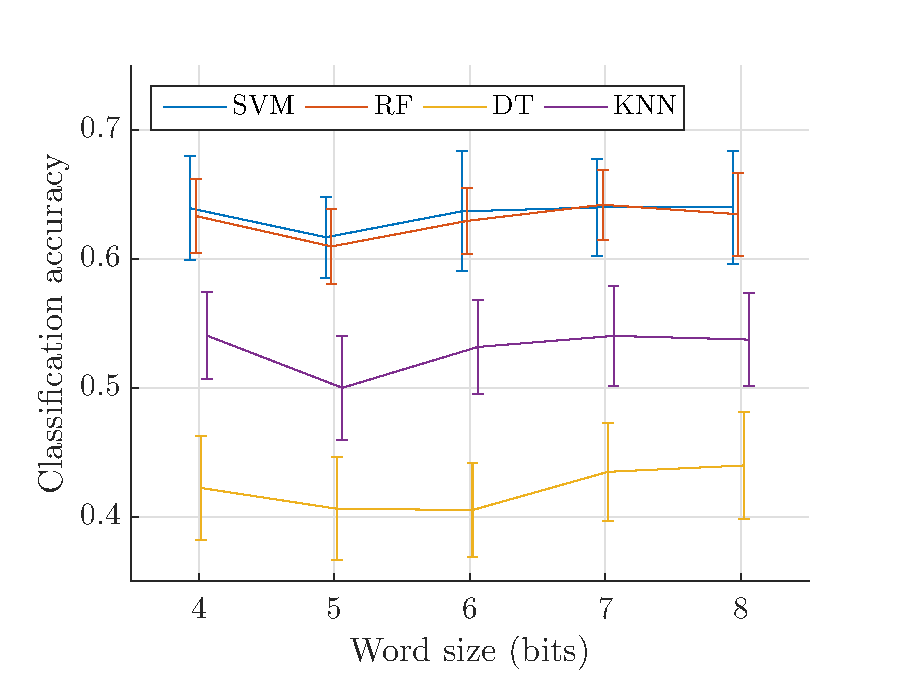
\includegraphics[width=\columnwidth]{figures/class_tob_q.eps}
	\caption{Classification accuracy with third-octave bands and varying word size.}
	\label{fig:class_tob_q}
\end{figure}

To further analyze both representations advantages, the confusion matrix is a reliable tool. It aims at providing information regarding class-by-class accuracy and misclassification rates. We thus compute these metrics for the SVM classifier, with predictions cumulated over the ten folds in test configuration. The analogous natures of the two descriptors is highlighted by close one-versus-one differentiation performances, with a slightly lower accuracy for third-octave bands on average. Both representations yield best results for the \textit{Gun shot} class with 88.2\% for third-octave cepstra and 86.6\% for mel cepstra. Their poorest accuracy is on the \textit{Air conditioning} class with 32.0\% and 38.1\% respectively. However, a noticeable difference between them is that on the log-frequency scale the bandwidth of mel filters narrows as frequency increases, while third-octave are evenly distributed. The effect of this can be seen between classes \textit{Drilling} and \textit{Jackhammer}. These sounds involve important low-frequency information which can generally differentiate them, leading third-octave descriptors to perform better. Conversely, using mel-based cepstra improves globally \textit{Air conditioning} recognition as most of its defining components are situated in higher frequencies.\\

Both descriptor are thus found to have similar representational capabilities despite minor construction differences.


\subsection{Inintelligibility}

Finally, objective intelligibility metrics are estimated for the studied parameters and compared to an informal perceptual evaluation \footnote{Decoded speech utterances for various conditions can be listened to at \url{http://}}. Figures~\ref{fig:csii_mel_avg} and \ref{fig:fwsnrseg_mel_avg} shows both the CSII and fwSNRseg indicators for varying representation dimensions. Figure~\ref{fig:percint_mel_avg} presents the results of the preliminar perceptual test for the same setup. %For this test, subjects were asked to blindly listen to recovered speech audio with different representation and coding parameters. They had to rate each extract between 0 ans 5, respectively inintelligible and perfectly comprehensible. We acknowledge that it is surely biased by a reduced number of participants and lack of tested audio material. However, it is sufficient to judge the relevance of objective indicators in our conditions as we can observe a correlation between the three metrics.

%The CSII accounts for the whole spectrogram distance between clean and distorted audio at each point in time and frequency. This includes the phase, which we discard early in the representation step. The error induced by forward and inverse mel bands transformation as well as operations reducing data dimensionality further contribute to very high distances. In fact, the signal is too distorted for the proposed SNR normalization to ensure CSII values in the 0-1 range. The indicator differs from perceptual evaluations for middle-valued frame rates, with for example the 9.5 fps curve being lower than expected. Values are also very close for multiple parameter combinations where a threshold between intelligibility and inintelligibility could be found. This is therefore not an adequate indicator for our purpose.\\

%Alternatively, the frequency-weighted segmental SNR considers only spectrogram magnitudes. As a result, distance is generally lower and a more representative of the induced perceptual distortion.  Nevertheless, the fwSNRseg still uses point-wise comparison. A shape seems to appear where the influences of frame rate and mel bands on output are decorrelated, ie. almost the same curve is offset as a function of frame rate. While the values are still concentrated around the critical threshold location at about -5~dB, this metric is likely a better indicator due to its approach of the clean-reconstructed signal distance. \ml{incrompehnsible}

\begin{figure}[htbp]
	\centering
		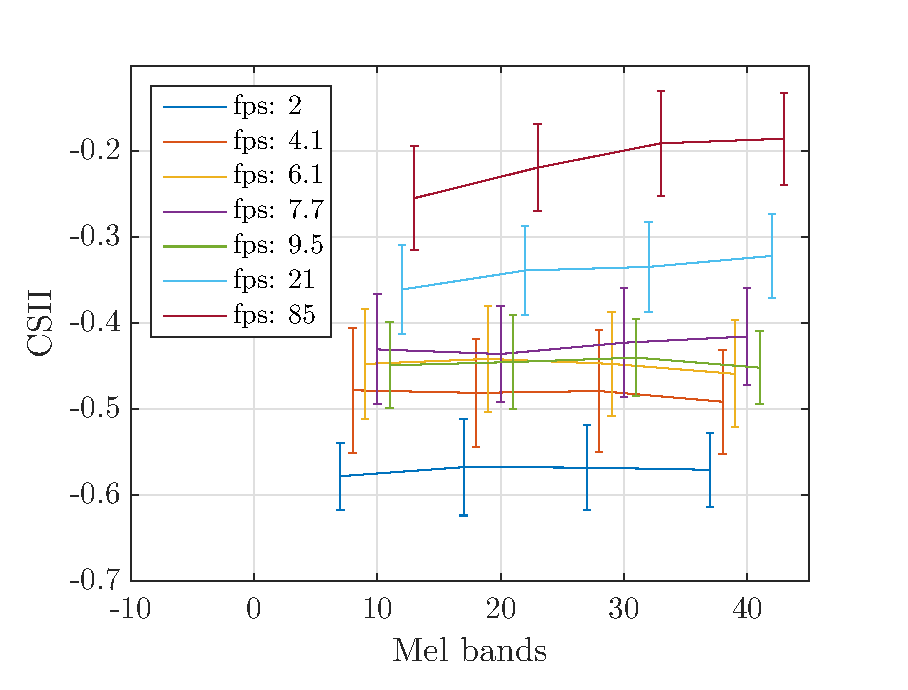
\includegraphics[width=\columnwidth]{figures/csii_mel_avg.eps}
	\caption{The Coherence SII objective indicator computed for intelligibility assessment. Negative CSII values indicate a signal-to-noise ratio too low for the recommended normalization, thus severe disparities between the original and reconstructed signal.}
	\label{fig:csii_mel_avg}
\end{figure}

\begin{figure}[htbp]
	\centering
		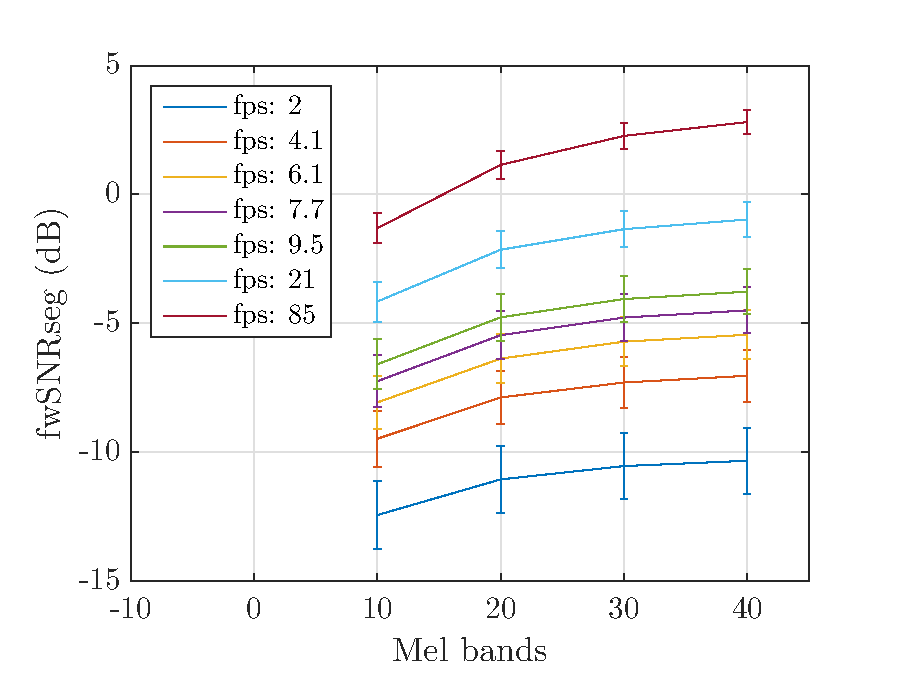
\includegraphics[width=\columnwidth]{figures/fwsnrseg_mel_avg.eps}
	\caption{Frequency-weighted segmental SNR for the same parameters.}
	\label{fig:fwsnrseg_mel_avg}
\end{figure}

\begin{figure}[htbp]
	\centering
		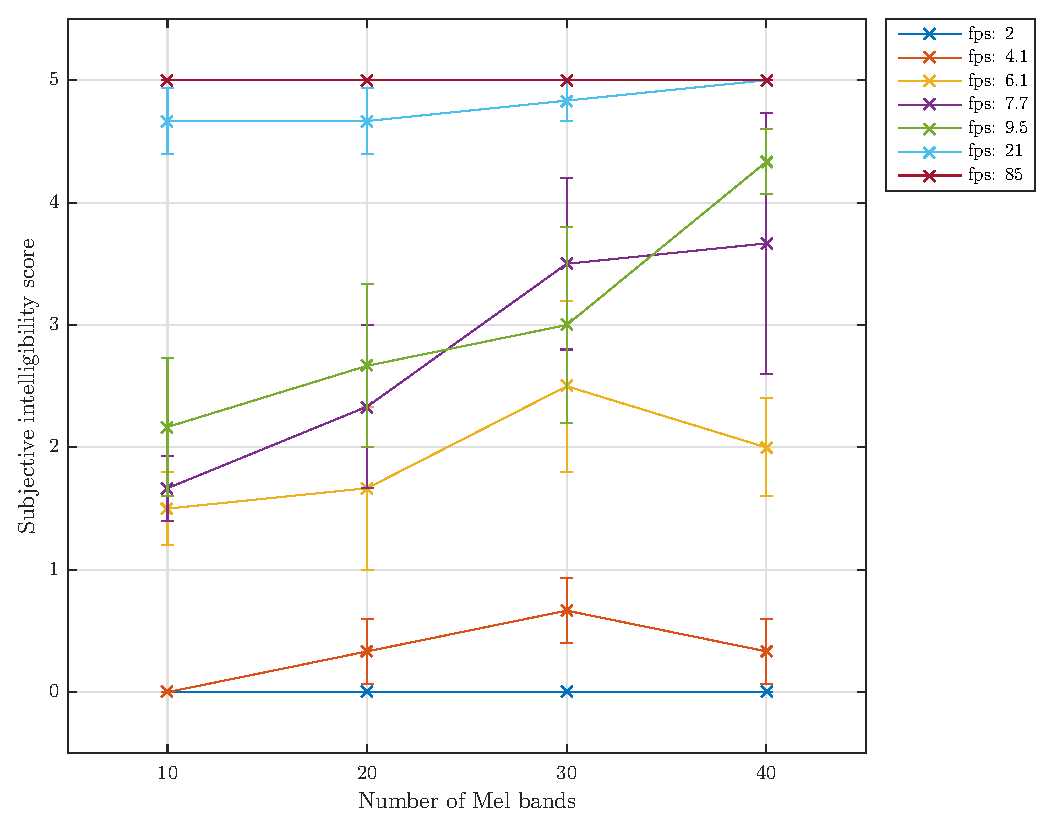
\includegraphics[width=\columnwidth]{figures/percint_mel_avg.eps}
	\caption{Results of the perceptual intelligibility test.}
	\label{fig:percint_mel_avg}
\end{figure}
\section{Conclusion}

\clearpage
%% The Appendices part is started with the command \appendix;
%% appendix sections are then done as normal sections
%% \appendix

%% \section{}
%% \label{}

%% If you have bibdatabase file and want bibtex to generate the
%% bibitems, please use
%%
%%  \bibliographystyle{elsarticle-harv}
%%  \bibliography{<your bibdatabase>}

%% else use the following coding to input the bibitems directly in the
%% TeX file.

\bibliographystyle{plain}
\bibliography{biblio}

%\ml{USE BIBTEX !!}
%\bibliography{mybib}{}
%
%
%\begin{thebibliography}{09}
%
%\bibitem{gozalo2015}
%Rey Gozalo, G. and Trujillo Carmona, J. and Barrigon Morillas, J.M. and Gomez Escobar, V. (2015). Relationship between objective acoustic indices and subjective assessments for the quality of soundscapes. \textit{Applied Acoustics}, 97, pp. 1-10
%
%\bibitem{rychtarikova2013}
%Rychtarikova, M. and Vermeir, G. (2013). Soundscape categorization on the basis of objective acoustical parameters. \textit{Applied Acoustics}, 74(2), pp. 240-247
%
%\bibitem{can2016}
%Can, A. and Aumond, P. and Michel, S. and De Coensel, B. and Ribeiro, C. and Botteldooren, D. and Lavandier, C. (2016). Comparison of noise indicators in an urban context. In: \textit{Proceedings of the 45th International Congress and Exposition on Noise Control Engineering}, pp. 5678-5686
%
%\bibitem{can2015}
%Can, A. and Gauvreau, B. (2015). Describing and classifying urban sound environments with a relevant set of physical indicators. \textit{J. Ac. Soc. Am.}, 137(1), pp. 208-218
%
%\bibitem{brocolini2013}
%Brocolini, L. and Lavandier, C. and Quoy, M. and Ribeiro, C. (2013). Measurements of acoustic environments for urban soundscapes: Choice of homogeneous periods, optimization of durations, and selection of indicators. \textit{J. Ac. Soc. Am.}, 134(1), pp. 813-821
%
%\bibitem{nilsson2007}
%Nilsson, M. and Botteldooren, D. and De Coensel, B. (2007). Acoustic indicators of soundscape quality and noise annoyance in outdoor urban areas. In: \textit{Proceedings of the 19th International Congress on Acoustics}
%
%\bibitem{ishiyama2000}
%Ishiyama, T. and Hashimoto, T. (2000). The impact of sound quality on annoyance caused by road traffc noise: an influence of frequency spectra on annoyance. \textit{JSAE Review}, 21(2), pp. 225-230
%
%\bibitem{torija2013}
%Torija, A. and Ruiz, D. and Ramos-Ridao, A. (2013). Application of a methodology for categorizing and differentiating urban soundscapes using acoustical descriptors and semantic-differential attributes. \textit{J. Ac. Soc. Am.}, 134(1), pp. 791-802
%
%\bibitem{anusuya2009}
%Anusuya, M. and Katty, S. (2009). Speech recognition by machine, a review. \textit{International Journal of Computer Science and Information Security}, 6(3), pp. 181-205
%
%\bibitem{tzanetakis2002}
%Tzanztakis, G. and Essl, G. and Cook, P. (2002). Automatic musical genre classification of audio signals. \textit{IEEE Transactions on Speech and Audio Processing}, 10(5), pp. 293-302
%
%\bibitem{ntalampiras2014}
%Ntalampiras, S. (2014). Universal background modeling for acoustic surveillance of urban traffic. \textit{Digital Signal Processing}, 31, pp. 69-78
%
%\bibitem{aucouturier2007}
%Aucouturier, J. and Defreville, B. and Pachet, F. (2007). The bag-of-frames approach to audio pattern recognition: A sufficient model for urban soundscapes but not for polyphonic music. \textit{J. Ac. Soc. Am.}, 122(2), pp. 881-891
%
%\bibitem{foggia2015}
%Foggia, P. and Petkov, N. and Saggese, A. and Strisciuglio, N. and Vento, M. (2015). Reliable detection of audio events in highly noisy environments. \textit{Pattern Recognition Letters}, 65, pp. 22-28
%
%\bibitem{kumar2016}
%Kumar, A. and Raj, B. (2016). Features and Kernels for Audio Event Recognition. \textit{arXiv Preprint}, Available at: \url{https://arxiv.org/abs/1607.05765}
%
%\bibitem{radhakrishnan2005}
%Radhakrishnan, R. and Divakaran, A. and Smaragdis, P. (2005). Audio analysis for surveillance applications. In: \textit{IEEE Workshop on Applications of Signal Processing to Audio and Acoustics}
%
%\bibitem{salamon2017}
%Salamon, J. and Bello, J. (2017). Deep convolutional neural networks and data augmentation for environmental sound classification. \textit{IEEE Signal Processing Letters}, 24(3), pp. 279-283
%
%\bibitem{piczak2015}
%Piczak, K. (2015). Environmental sound classification with convolutional neural networks. In: \textit{IEEE 25th International Workshop on Machine Learning for Signal Processing}
%
%\bibitem{khunarsal2013}
%Khunarsal, P. and Lursinsap, C. and Raicharoen, T. (2013). Very short time environmental sound classification based on spectrogram pattern matching. \textit{Information Sciences}, 243, pp. 57-74
%
%\bibitem{couvreur2004}
%Couvreur, L. and Laniray, M. (2004). Automatic noise recognition in urban environments based on artificial neural networks and hidden markov models. In: \textit{The 33rd International Congress and Exposition on Noise Control Engineering}
%
%\bibitem{cai2006}
%Cai, R. and Lu, L. and Hanjalic, A. and Zhang, H. and Cai, L. (2006). A flexible framewok for key audio effects detection and auditory context inference. \textit{IEEE Transactions on Audio, Speech, and Language Processing}, 14(3), pp. 1026-1039
%
%\bibitem{chu2009}
%Chu, S. and Narayanan, S. and Kuo, C. (2009). Environmental sound recognition with time-frequency audio features. \textit{IEEE Transactions on Audio, Speech, and Language Processing}, 17(6), pp. 1142-1158
%
%\bibitem{salamon2015-2}
%Salamon, J. and Bello, J. (2015). Unsupervised feature learning for urman sound classification. In: \textit{2015 IEEE International Conference on Acoustics, Speech and Signal Processing}
%
%\bibitem{bauge2013}
%Baugé, C. and Lagrange, M. and Andén, J. and Mallat, S. (2013). Representing environmental sounds using the separable scattering transform. In: \textit{2013 IEEE International Conference on Acoustics, Speech and Signal Processing}
%
%\bibitem{salamon2015}
%Salamon, J. and Bello, J. (2015). Feature learning with deep scattering for urban sound analysis. In: \textit{23rd European Signal Processing Conference}
%
%\bibitem{chachada2013}
%Chachada, S. and Kuo, C. (2013). Environmental sound recognition: A survey. In: \textit{2013 Asia-Pacific Signal and Information Processing Association Annual Summit and Conference}
%
%\bibitem{davis1986}
%Davis, S. (1986). Octave and fractional-octave band digital filtering based on the proposed ANSI standard. In: \textit{1986 IEEE International Conference on Acoustics, Speech and Signal Processing}
%
%\bibitem{ellis2005}
%Ellis, D. (2005). \textit{{PLP} and {RASTA} (and {MFCC}, and inversion) in {M}atlab}. Available at: \url{http://www.ee.columbia.edu/~dpwe/resources/matlab/rastamat/}
%
%\bibitem{huffman1952}
%Huffman, D. (1952). A method for the construction of minimum-redundancy codes. \textit{Proceedings of the IRE}, 40(9), pp. 1098-1101
%
%\bibitem{antoni2010}
%Antoni, J. (2010). Orthogonal-like fractional-octave-band filters. \textit{J. Ac. Soc. Am.}, 127(2), pp. 884–895
%
%\bibitem{couvreur}
%Couvreur, C. \textit{Implementation of a one-third-octave filter bank in Matlab}. Available at: \url{http://citeseer.ist.psu.edu/24150.html}
%
%\bibitem{griffin1984}
%Griffin, D. and Lim, J. (1984). Signal Estimation from Modified Short-Time Fourier Transform. \textit{IEEE Transactions on Acoustics, Speech, and Signal Processing}, 32(2), pp. 236-243
%
%\bibitem{salamon2014}
%Salamon, J. and Jacoby, C. and Bello, J. (2014). A Dataset and Taxonomy for Urban Sound Research. \textit{Proceedings of the 22nd ACM international conference on Multimedia}
%
%\bibitem{kates2005}
%Kates, J. and Arehart, K. (2005). Coherence and the Speech Intelligibility Index. \textit{J. Ac. Soc. Am.}, 115(5), pp. 2224–2237
%
%\bibitem{hu2008}
%Hu, Y. and Loizou, P. (2008). Evaluation of objective quality measures for speech enhancement. \textit{IEEE Transactions on Audio, Speech, and Language Processing}, 16(1), pp. 229–238
%
%\bibitem{ma2009}
%Ma, J. and Hu, Y. and Loizou, P. (2009). Objective measures for predicting speech intelligibility in noisy conditions based on new band-importance functions. \textit{J. Ac. Soc. Am.}, 125(5), pp. 3387–3405
%
%
%\end{thebibliography}
\end{document}

\endinput
%%
%% End of file `elsarticle-template-harv.tex'.
